%% Author_tex.tex
%% V1.0
%% 2012/13/12
%% developed by Techset
%%
%% This file describes the coding for modeloUFCG.cls

%% O Quarto copia os arquivos de suporte da extensao (resources: no
%% _extension.yml) preservando o caminho relativo _extensions/modeloufcg/,
%% entao o .cls, o .bst e o logo sao referenciados com esse prefixo.
\documentclass[a4paper]{_extensions/modeloufcg/modeloUFCG}

\usepackage[portuguese]{babel}
\usepackage[T1]{fontenc}
\usepackage[utf8]{inputenc}
\usepackage{fancyhdr}
\usepackage{booktabs}
\usepackage{longtable}
\newcounter{none} % tabelas sem legenda numerada (usado pelo Quarto/crossref)
\usepackage{array}
\usepackage{calc}
%% Fixa cada figura exatamente onde e gerada ([H]). Sem isso, floats podem
%% "flutuar" livremente e, neste documento (muitas figuras grandes em
%% sequencia), acabam se deslocando para muito longe do texto que os
%% referencia -- inclusive interferindo na quebra de pagina de tabelas
%% longtable vizinhas.
\usepackage{float}

%% A classe modeloUFCG.cls calcula largura/altura de texto e margens
%% assumindo o formato de trim de um periodico (174mm x 247mm), mas o PDF
%% final e produzido em A4 (210mm x 297mm). Isso deixa sobras enormes nas
%% margens. O pacote geometry forca margens A4 corretas, sobrepondo o
%% calculo original da classe.
\usepackage[a4paper, margin=2.5cm]{geometry}

\pagestyle{fancy}
\renewcommand{\headrulewidth}{0pt}
\fancyhead[L]{}
\fancyhead[C]{}
\fancyhead[R]{}

%% A classe usa \flushbottom, que estica os espacos em branco de cada pagina
%% para preenche-la ate o final. Combinado com figuras fixas ([H]), isso cria
%% buracos enormes entre uma figura/tabela e o texto seguinte. \raggedbottom
%% deixa o espaco sobrando apenas no rodape da pagina, sem esticar o meio.
\raggedbottom

%% Espacamento mais enxuto ao redor de figuras e tabelas.
\setlength{\floatsep}{8pt plus 2pt minus 2pt}
\setlength{\textfloatsep}{10pt plus 2pt minus 2pt}
\setlength{\intextsep}{8pt plus 2pt minus 2pt}

\makeatletter
\@ifpackageloaded{caption}{}{\usepackage{caption}}
\AtBeginDocument{%
\ifdefined\contentsname
  \renewcommand*\contentsname{Table of contents}
\else
  \newcommand\contentsname{Table of contents}
\fi
\ifdefined\listfigurename
  \renewcommand*\listfigurename{List of Figures}
\else
  \newcommand\listfigurename{List of Figures}
\fi
\ifdefined\listtablename
  \renewcommand*\listtablename{List of Tables}
\else
  \newcommand\listtablename{List of Tables}
\fi
\ifdefined\figurename
  \renewcommand*\figurename{Figure}
\else
  \newcommand\figurename{Figure}
\fi
\ifdefined\tablename
  \renewcommand*\tablename{Table}
\else
  \newcommand\tablename{Table}
\fi
}
\@ifpackageloaded{float}{}{\usepackage{float}}
\floatstyle{ruled}
\@ifundefined{c@chapter}{\newfloat{codelisting}{h}{lop}}{\newfloat{codelisting}{h}{lop}[chapter]}
\floatname{codelisting}{Listing}
\newcommand*\listoflistings{\listof{codelisting}{List of Listings}}
\makeatother
\makeatletter
\makeatother
\makeatletter
\@ifpackageloaded{caption}{}{\usepackage{caption}}
\@ifpackageloaded{subcaption}{}{\usepackage{subcaption}}
\makeatother

%%%% *** Do not adjust lengths that control margins, column widths, etc. ***

%%%%%%%%%%% Defining Enunciations  %%%%%%%%%%%
\newtheorem{theorem}{\bf Teorema}[section]
\newtheorem{condition}{\bf Condição}[section]
\newtheorem{corollary}{\bf Corolário}[section]
%%%%%%%%%%%%%%%%%%%%%%%%%%%%%%%%%%%%%%%%%%%%%%%

\usepackage{titlesec}
\renewcommand{\thesection}{\arabic{section}}
\renewcommand{\thesubsection}{\thesection.\arabic{subsection}}
\renewcommand{\thesubsubsection}{\thesubsection.\arabic{subsubsection}}

%%%% Cabecalho no estilo de artigo academico, substituindo a capa           %%%%
%%%% original (logo + caixa de titulo) do template Royal Society.          %%%%
%%%% A caixa de resumo estreita e trocada por um resumo de largura total,  %%%%
%%%% exibido logo apos o titulo/autores, como em um artigo convencional.   %%%%
%% Apos o \documentclass terminar de carregar, o LaTeX restaura o catcode de
%% @ para "outro", entao qualquer referencia a comandos internos da classe
%% (\@title, \@author, \if@subject@provided etc.) precisa ficar dentro de
%% \makeatletter ... \makeatother para ser reconhecida corretamente.
\makeatletter

%% Centraliza as legendas de figuras e tabelas (a classe original as deixa
%% alinhadas a esquerda).
\long\def\@makecaption#1#2{%
  \vskip\abovecaptionskip
  \centering{\captionheadfont #1.}\hskip2.5pt{\captionfont #2}\par
  \vskip\belowcaptionskip}

\renewenvironment{abstract}{%
  \global\setbox\absbox\vbox\bgroup\par\abstractfont
  \leftskip0pc\rightskip0pc\noindent\ignorespaces
}{\par\egroup}

%% A classe modeloUFCG.cls define \@maketitle atraves de mecanismos internos
%% (fila de duas colunas / bloco de revisao editorial) que absorvem qualquer
%% redefinicao de \@maketitle sem executa-la. Para evitar essa maquinaria,
%% \maketitle e redefinido diretamente aqui.
\renewcommand\maketitle{%
  \vspace*{-2.2cm}
  \noindent\begin{minipage}[c]{2.2cm}
    
\includegraphics[width=2cm]{_extensions/modeloufcg/lea_logo_bw}
  \end{minipage}%
  \begin{minipage}[c]{\textwidth-2.2cm}
    {\fontfamily{\sfdefault}\fontseries{b}\fontshape{n}\fontsize{12}{14}\selectfont
      UNIVERSIDADE FEDERAL DE CAMPINA GRANDE\par}
          {\fontfamily{\sfdefault}\fontseries{m}\fontshape{n}\fontsize{11}{13}\selectfont
       Disciplina: Estatística Aplicada%
        \quad---\quad Período: 2026.1\par}
              {\fontfamily{\sfdefault}\fontseries{m}\fontshape{n}\fontsize{11}{13}\selectfont
       Professores: Prof.~Gilberto Matos; Profa. Amanda Gomes\par}
      \end{minipage}
  \vskip4pt
  \rule{\textwidth}{.5pt}
  \vskip8pt
  \begin{center}
    {\fontfamily{\sfdefault}\fontseries{m}\fontshape{n}\fontsize{16}{18}\selectfont\mathversion{bold}\@title\par}
    \vskip6pt
    {\authorfont\@author\par}
    \vskip3pt
    \ifx\@address\empty\else
      {\addressfont\@address\par}
    \fi
    \vskip6pt
    \rule{\textwidth}{.5pt}
  \end{center}
  \vskip8pt
  \ifvoid\absbox\else
    {\fontfamily{\sfdefault}\fontseries{b}\fontshape{n}\fontsize{11}{13}\selectfont Resumo}\par
    \vskip4pt
    \noindent\usebox\absbox\par
    \vskip6pt
  \fi
  \if@subject@provided
    {\subjectfont\@subject\par}
    \vskip4pt
  \fi
  \if@keywords@provided
    {\keywordfont\@keywords\par}
  \fi
  \vskip10pt
}

\makeatother

\begin{document}

%%%% Article title to be placed here
\title{Modelagem do Comprimento da Sépala em Flores do Gênero Iris}

\author{
$^{}$}

\address{
  $^{1}$Departamento de Ciência da Computação - UFCG}
%%%% Subject entries to be placed here %%%%
\subject{
estatística aplicada,
modelagem preditiva}

%%%% Keyword entries to be placed here %%%%
\keywords{
regressão linear múltipla,
multicolinearidade,
seleção de modelos,
variáveis dummy}

%%%% Abstract text to be placed here %%%%%%%%%%%%
\begin{abstract}
Analisamos a base \texttt{iris} sob a ótica de um modelo de regressão
linear múltipla, utilizando o comprimento da sépala
(\texttt{Sepal.Length}) como variável resposta. Após identificar
multicolinearidade severa entre \texttt{Petal.Length} e
\texttt{Petal.Width} via VIF, selecionamos um modelo mais parcimonioso
por AIC/BIC e teste F, verificamos seus pressupostos e avaliamos o
efeito de incorporar a espécie como variável explicativa qualitativa,
incluindo a técnica de variáveis dummy e a escolha de categoria de
referência.
\end{abstract}
%%%%%%%%%%%%%%%%%%%%%%%%%%%

%% Some pieces required from the pandoc template
\providecommand{\tightlist}{%
  \setlength{\itemsep}{0pt}\setlength{\parskip}{0pt}}
\providecommand{\EndFirstPage}{%
}
%% O Quarto (ao contrario do fluxo R Markdown, que usa --no-highlight) sempre
%% injeta \pandocbounded ao redor de imagens; a classe nao o define.
\providecommand{\pandocbounded}[1]{#1}

\maketitle

\section{Introdução}\label{introduuxe7uxe3o}

O conjunto de dados \texttt{iris} \citep{Fisher1936, Anderson1935} reúne
150 observações de flores de três espécies do gênero \emph{Iris}
(\emph{setosa}, \emph{versicolor} e \emph{virginica}), com quatro
medidas morfológicas por flor. Neste relatório, tratamos o comprimento
da sépala (\texttt{Sepal.Length}) como variável resposta e as demais
medidas contínuas, além da espécie, como candidatas a variáveis
explicativas, com o objetivo de construir um modelo de regressão linear
múltipla parcimonioso e adequado aos dados.

\section{Metodologia}\label{metodologia}

\subsection{Modelo de regressão linear
múltipla}\label{modelo-de-regressuxe3o-linear-muxfaltipla}

Ajustamos inicialmente um modelo com as três variáveis contínuas
disponíveis (\texttt{Sepal.Width}, \texttt{Petal.Length} e
\texttt{Petal.Width}). Como estas variáveis morfológicas tendem a ser
correlacionadas entre si, avaliamos a multicolinearidade por meio do
fator de inflação de variância (VIF), usando como referência o limiar
informal de 10 \citep{Kutner2004}. A seleção do modelo final combina os
critérios AIC \citep{Akaike1974} e BIC \citep{Schwarz1978}, além de
testes F aninhados.

\subsection{Diagnóstico do modelo}\label{diagnuxf3stico-do-modelo}

Os pressupostos de linearidade, homocedasticidade e normalidade dos
erros são avaliados por meio de gráficos de resíduos e de um envelope
simulado \citep{CookWeisberg1982}. Pontos atípicos, de alavanca e
influentes são identificados via resíduos estudentizados, alavancagem e
distância de Cook \citep{Cook1977}.

\subsection{Variáveis dummy e categoria de
referência}\label{variuxe1veis-dummy-e-categoria-de-referuxeancia}

Como \texttt{Species} é uma variável categórica com três níveis, sua
inclusão no modelo é feita por codificação dummy (duas colunas
indicadoras), e discutimos como a escolha da categoria de referência
afeta apenas a interpretação dos coeficientes, não os valores preditos.

\subsection{Inferência preditiva}\label{inferuxeancia-preditiva}

Por fim, ilustramos a diferença prática entre um intervalo de confiança
para o valor médio da resposta e um intervalo de predição para uma nova
observação individual.

\section{Resultados}\label{resultados}

\subsection{Descrição da base de
dados}\label{descriuxe7uxe3o-da-base-de-dados}

{

\begin{longtable}[]{@{}ll@{}}

\caption{\label{tbl-descricao}Variáveis da base de dados iris.}

\tabularnewline

\toprule\noalign{}
Variável & Descrição \\
\midrule\noalign{}
\endhead
\bottomrule\noalign{}
\endlastfoot
Sepal.Length & Comprimento da sépala (cm) \\
Sepal.Width & Largura da sépala (cm) \\
Petal.Length & Comprimento da pétala (cm) \\
Petal.Width & Largura da pétala (cm) \\
Species & Espécie (setosa, versicolor, virginica) \\

\end{longtable}

}

A base contém \(n=150\) observações, 50 para cada uma das três espécies,
sem dados ausentes.

\subsection{Análise exploratória}\label{anuxe1lise-exploratuxf3ria}

{

\begin{longtable}[]{@{}lllll@{}}

\caption{\label{tbl-descritivas}Estatísticas descritivas das variáveis
contínuas.}

\tabularnewline

\toprule\noalign{}
& mean & std & min & max \\
\midrule\noalign{}
\endhead
\bottomrule\noalign{}
\endlastfoot
Sepal.Length & 5.84 & 0.83 & 4.3 & 7.9 \\
Sepal.Width & 3.06 & 0.44 & 2.0 & 4.4 \\
Petal.Length & 3.76 & 1.77 & 1.0 & 6.9 \\
Petal.Width & 1.20 & 0.76 & 0.1 & 2.5 \\

\end{longtable}

}

\begin{figure}

\centering{

\pandocbounded{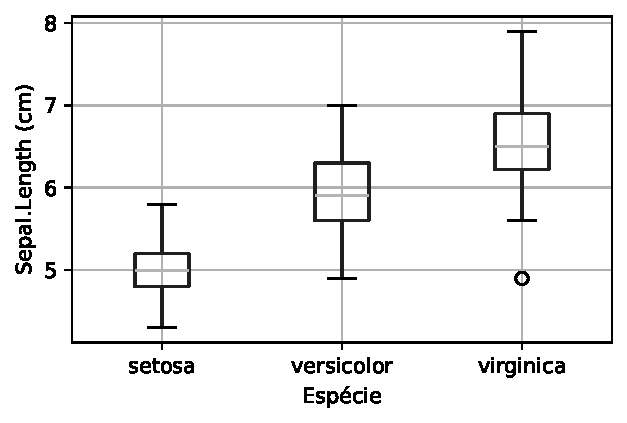
\includegraphics[keepaspectratio]{relatorio_files/figure-pdf/fig-boxplots-output-1.pdf}}

}

\caption{\label{fig-boxplots}Distribuição do comprimento da sépala por
espécie.}

\end{figure}%

A Figura \ref{fig-boxplots} sugere que \emph{virginica} tende a ter
sépalas mais compridas, seguida por \emph{versicolor} e, por último,
\emph{setosa}.

\subsubsection{Análise de
correlação}\label{anuxe1lise-de-correlauxe7uxe3o}

\begin{figure}

\centering{

\pandocbounded{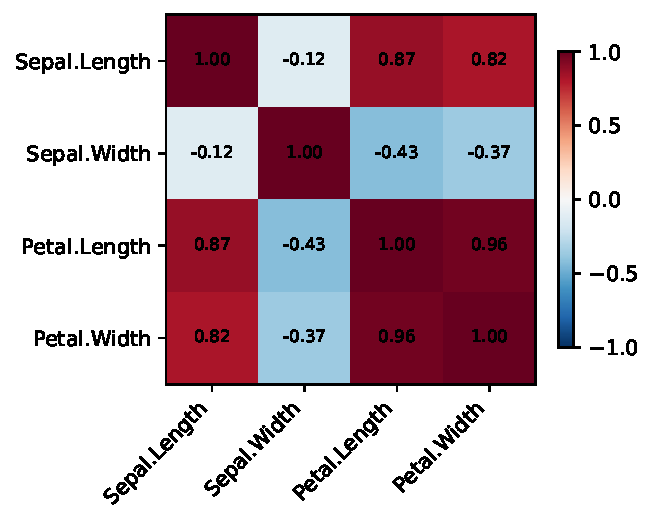
\includegraphics[keepaspectratio]{relatorio_files/figure-pdf/fig-corr-output-1.pdf}}

}

\caption{\label{fig-corr}Matriz de correlação de Pearson entre as
variáveis morfológicas.}

\end{figure}%

A variável resposta \texttt{Sepal.Length} não apresenta correlação
linear relevante com \texttt{Sepal.Width} (\(r \approx -0{,}12\)), mas
correlaciona-se fortemente com \texttt{Petal.Length}
(\(r \approx 0{,}87\)) e \texttt{Petal.Width} (\(r \approx 0{,}82\)).
Entre as próprias explicativas, \texttt{Petal.Length} e
\texttt{Petal.Width} apresentam correlação muito forte
(\(r \approx 0{,}96\)), o que já é um indício de multicolinearidade a
ser confirmado pelo VIF.

\subsubsection{Multicolinearidade: o
VIF}\label{multicolinearidade-o-vif}

{

\begin{longtable}[]{@{}lllllll@{}}

\caption{\label{tbl-modelocompleto}Estimativas do modelo inicial (sem a
espécie).}

\tabularnewline

\toprule\noalign{}
& Coef. & Std.Err. & t & P\textgreater\textbar t\textbar{} & {[}0.025 &
0.975{]} \\
\midrule\noalign{}
\endhead
\bottomrule\noalign{}
\endlastfoot
Intercept & 1.8560 & 0.2508 & 7.4010 & 0.0 & 1.3604 & 2.3516 \\
Q(\textquotesingle Sepal.Width\textquotesingle) & 0.6508 & 0.0666 &
9.7654 & 0.0 & 0.5191 & 0.7826 \\
Q(\textquotesingle Petal.Length\textquotesingle) & 0.7091 & 0.0567 &
12.5025 & 0.0 & 0.5970 & 0.8212 \\
Q(\textquotesingle Petal.Width\textquotesingle) & -0.5565 & 0.1275 &
-4.3629 & 0.0 & -0.8086 & -0.3044 \\

\end{longtable}

}

{

\begin{longtable}[]{@{}ll@{}}

\caption{\label{tbl-vif}Fator de inflação de variância (VIF) de cada
variável explicativa no modelo inicial.}

\tabularnewline

\toprule\noalign{}
& VIF \\
\midrule\noalign{}
\endhead
\bottomrule\noalign{}
\endlastfoot
Sepal.Width & 1.27 \\
Petal.Length & 15.10 \\
Petal.Width & 14.23 \\

\end{longtable}

}

O modelo inicial apresenta ajuste elevado (\(R^2\) ajustado \(=\)
0.8557), mas o VIF de \texttt{Petal.Length} e \texttt{Petal.Width}
(acima de 14) confirma multicolinearidade severa entre essas duas
variáveis, muito acima do limiar de referência de 10. Um segundo indício
é o sinal negativo do coeficiente de \texttt{Petal.Width},
contraintuitivo dado que ambas as variáveis se correlacionam
positivamente com a resposta: consequência típica de multicolinearidade,
que torna as estimativas individuais instáveis mesmo com o ajuste global
permanecendo bom.

\subsection{Seleção do modelo
final}\label{seleuxe7uxe3o-do-modelo-final}

{

\begin{longtable}[]{@{}lrrr@{}}

\caption{\label{tbl-selecao}Comparação dos modelos candidatos: ajuste,
AIC e BIC.}

\tabularnewline

\toprule\noalign{}
Modelo & R² ajustado & AIC & BIC \\
\midrule\noalign{}
\endhead
\bottomrule\noalign{}
\endlastfoot
modelo1 (completo) & 0.86 & 82.64 & 94.69 \\
modelo2 (sem Petal.Width) & 0.84 & 99.03 & 108.06 \\
modelo3 (sem Petal.Length) & 0.7 & 189.82 & 198.85 \\

\end{longtable}

}

O modelo2 (sem \texttt{Petal.Width}) apresenta AIC e BIC menores que o
modelo3, com diferença muito superior a 10 em ambos os critérios,
evidência forte de que é o modelo preferível. Isto é coerente com a
análise de correlação: \texttt{Petal.Width} correlaciona-se um pouco
menos com a resposta do que \texttt{Petal.Length}, de modo que, entre as
duas variáveis colineares, é preferível manter a mais associada a
\texttt{Sepal.Length}.

{

\begin{longtable}[]{@{}
  >{\raggedright\arraybackslash}p{(\linewidth - 12\tabcolsep) * \real{0.1351}}
  >{\raggedleft\arraybackslash}p{(\linewidth - 12\tabcolsep) * \real{0.1486}}
  >{\raggedleft\arraybackslash}p{(\linewidth - 12\tabcolsep) * \real{0.1486}}
  >{\raggedleft\arraybackslash}p{(\linewidth - 12\tabcolsep) * \real{0.0811}}
  >{\raggedleft\arraybackslash}p{(\linewidth - 12\tabcolsep) * \real{0.1081}}
  >{\raggedleft\arraybackslash}p{(\linewidth - 12\tabcolsep) * \real{0.2297}}
  >{\raggedleft\arraybackslash}p{(\linewidth - 12\tabcolsep) * \real{0.1486}}@{}}

\caption{\label{tbl-anova2}Teste F comparando o modelo2 ao modelo
completo (modelo1).}

\tabularnewline

\toprule\noalign{}
\begin{minipage}[b]{\linewidth}\raggedright
Modelo
\end{minipage} & \begin{minipage}[b]{\linewidth}\raggedleft
GL Res.
\end{minipage} & \begin{minipage}[b]{\linewidth}\raggedleft
SQ Res.
\end{minipage} & \begin{minipage}[b]{\linewidth}\raggedleft
GL
\end{minipage} & \begin{minipage}[b]{\linewidth}\raggedleft
SQ
\end{minipage} & \begin{minipage}[b]{\linewidth}\raggedleft
Estatística F
\end{minipage} & \begin{minipage}[b]{\linewidth}\raggedleft
p-valor
\end{minipage} \\
\midrule\noalign{}
\endhead
\bottomrule\noalign{}
\endlastfoot
modelo2 & 147 & 16.3288 & 0 & & & \\
modelo1 & 146 & 14.4454 & 1 & 1.8834 & 19.0352 & 0 \\

\end{longtable}

}

O teste F rejeita a hipótese nula de que o submodelo sem
\texttt{Petal.Width} explica tão bem quanto o modelo completo
(\(p<0{,}001\)), ou seja, a variável é individualmente significante,
ainda que sua presença simultânea com \texttt{Petal.Length} cause o
problema de multicolinearidade discutido acima.

\subsubsection{Seleção automática (eliminação retroativa por
AIC)}\label{seleuxe7uxe3o-automuxe1tica-eliminauxe7uxe3o-retroativa-por-aic}

O \texttt{statsmodels} não possui uma função equivalente ao
\texttt{step()} do R; reproduzimos a mesma lógica de eliminação
retroativa manualmente, removendo a cada passo a variável cuja remoção
resulta no maior ganho de AIC, e parando quando nenhuma remoção melhora
o critério:

\begin{verbatim}
def selecao_retroativa(formula_completa, dados, resposta):
    termos = formula_completa
    modelo_atual = smf.ols(f"Q('{resposta}') ~ " + " + ".join(f"Q('{t}')" for t in termos),
                            data=dados).fit()
    print(f"Início: AIC = {modelo_atual.aic:.2f}  |  termos: {termos}")
    while True:
        aics = {}
        for termo in termos:
            restantes = [t for t in termos if t != termo]
            f = f"Q('{resposta}') ~ " + " + ".join(f"Q('{t}')" for t in restantes)
            aics[termo] = smf.ols(f, data=dados).fit().aic
        melhor_termo = min(aics, key=aics.get)
        if aics[melhor_termo] >= modelo_atual.aic:
            print("Nenhuma remoção melhora o AIC. Processo encerrado.")
            break
        termos = [t for t in termos if t != melhor_termo]
        modelo_atual = smf.ols(f"Q('{resposta}') ~ " + " + ".join(f"Q('{t}')" for t in termos),
                                data=dados).fit()
        print(f"- Remove {melhor_termo}: AIC = {modelo_atual.aic:.2f}  |  termos: {termos}")
    return modelo_atual

_ = selecao_retroativa(["Sepal.Width", "Petal.Length", "Petal.Width"], dados, "Sepal.Length")
\end{verbatim}

\begin{verbatim}
Início: AIC = 82.64  |  termos: ['Sepal.Width', 'Petal.Length', 'Petal.Width']
Nenhuma remoção melhora o AIC. Processo encerrado.
\end{verbatim}

Assim como no procedimento \texttt{stepwise} do R, o critério puramente
preditivo (AIC) não recomenda a remoção de nenhuma variável: o modelo
completo já é o ótimo local por esse critério, mesmo colinear. Como o
objetivo aqui inclui interpretar os efeitos individuais, optamos por
seguir com o modelo2, que resolve a multicolinearidade a um custo mínimo
de ajuste (Tabela \ref{tbl-selecao}).

\subsection{Diagnóstico do modelo
selecionado}\label{diagnuxf3stico-do-modelo-selecionado}

{

\begin{longtable}[]{@{}lllllll@{}}

\caption{\label{tbl-modelo2}Estimativas dos coeficientes do modelo2
(modelo selecionado).}

\tabularnewline

\toprule\noalign{}
& Coef. & Std.Err. & t & P\textgreater\textbar t\textbar{} & {[}0.025 &
0.975{]} \\
\midrule\noalign{}
\endhead
\bottomrule\noalign{}
\endlastfoot
Intercept & 2.2491 & 0.2480 & 9.0702 & 0.0 & 1.7591 & 2.7392 \\
Q(\textquotesingle Sepal.Width\textquotesingle) & 0.5955 & 0.0693 &
8.5899 & 0.0 & 0.4585 & 0.7325 \\
Q(\textquotesingle Petal.Length\textquotesingle) & 0.4719 & 0.0171 &
27.5692 & 0.0 & 0.4381 & 0.5057 \\

\end{longtable}

}

\begin{figure}

\centering{

\pandocbounded{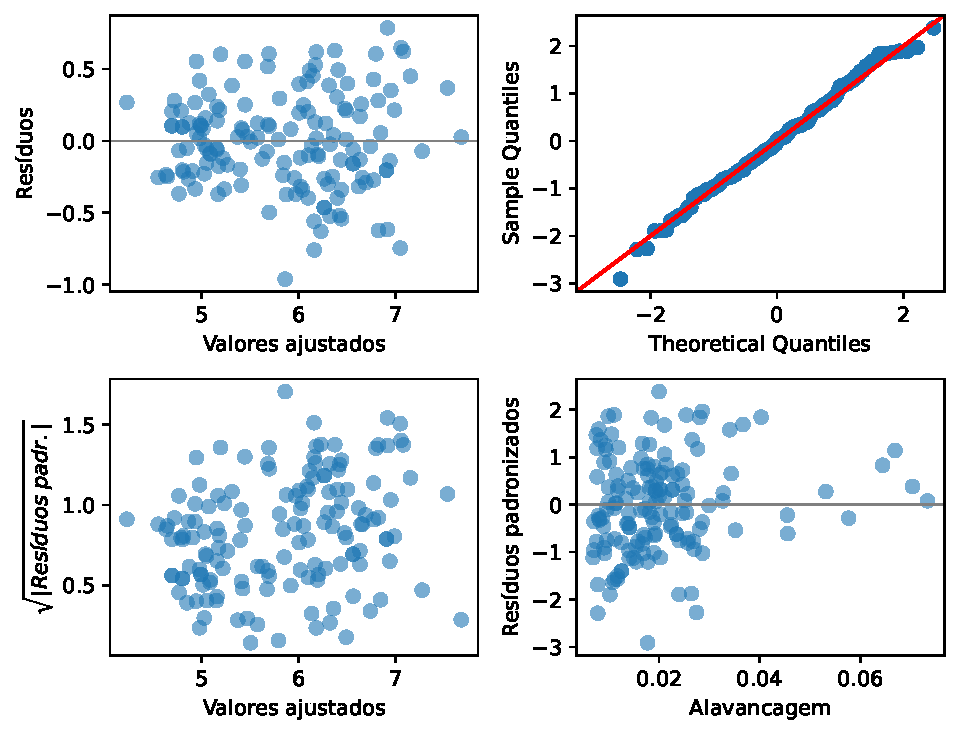
\includegraphics[keepaspectratio]{relatorio_files/figure-pdf/fig-diagnostico-output-1.pdf}}

}

\caption{\label{fig-diagnostico}Análise de resíduos do modelo2.}

\end{figure}%

\begin{figure}

\centering{

\pandocbounded{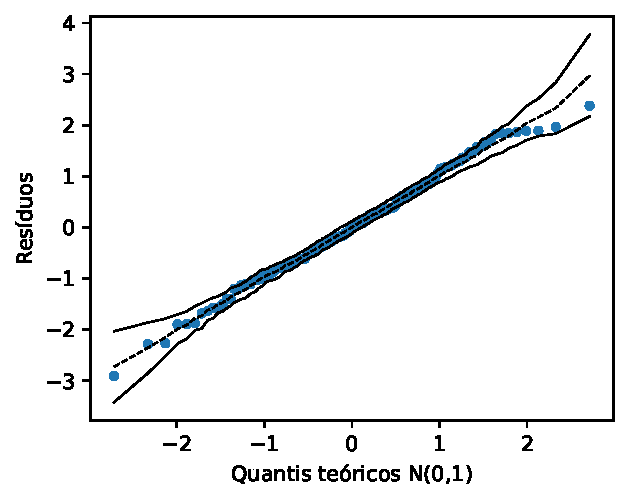
\includegraphics[keepaspectratio]{relatorio_files/figure-pdf/fig-envelope-output-1.pdf}}

}

\caption{\label{fig-envelope}Gráfico de envelope simulado do modelo2.}

\end{figure}%

As Figuras \ref{fig-diagnostico} e \ref{fig-envelope} não indicam
padrões sistemáticos relevantes nos resíduos, e a grande maioria dos
pontos permanece dentro da banda do envelope simulado, dando suporte às
suposições de linearidade, variância constante e normalidade dos erros.

\subsubsection{Identificação de pontos atípicos, de alavanca e
influentes}\label{identificauxe7uxe3o-de-pontos-atuxedpicos-de-alavanca-e-influentes}

{

\begin{longtable}[]{@{}llllllll@{}}

\caption{\label{tbl-influencia}Observações atípicas, de alavanca e/ou
influentes segundo o modelo2.}

\tabularnewline

\toprule\noalign{}
& Espécie & Resíduo estud. & Alavancagem & Dist. de Cook & Atípico &
Alavanca & Influente \\
\midrule\noalign{}
\endhead
\bottomrule\noalign{}
\endlastfoot
106 & virginica & -2.9112 & 0.0178 & 0.0511 & True & False & True \\
100 & virginica & -2.2694 & 0.0275 & 0.0485 & True & False & True \\
14 & setosa & 1.8452 & 0.0403 & 0.0477 & False & True & True \\
135 & virginica & 2.3810 & 0.0200 & 0.0387 & True & False & True \\
118 & virginica & 1.9674 & 0.0286 & 0.0380 & False & False & True \\
62 & versicolor & 1.6906 & 0.0367 & 0.0363 & False & False & True \\
87 & versicolor & 1.8404 & 0.0281 & 0.0327 & False & False & True \\
136 & virginica & -1.8753 & 0.0265 & 0.0319 & False & False & True \\
131 & virginica & 1.1417 & 0.0669 & 0.0312 & False & True & True \\
122 & virginica & 1.8890 & 0.0254 & 0.0310 & False & False & True \\
148 & virginica & -1.8900 & 0.0240 & 0.0293 & False & False & True \\
68 & versicolor & 1.5786 & 0.0341 & 0.0293 & False & False & True \\
41 & setosa & 0.8303 & 0.0645 & 0.0158 & False & True & False \\
84 & versicolor & -2.2874 & 0.0079 & 0.0138 & True & False & False \\
32 & setosa & -0.6102 & 0.0456 & 0.0059 & False & True & False \\
15 & setosa & 0.3817 & 0.0704 & 0.0037 & False & True & False \\
60 & versicolor & -0.2841 & 0.0577 & 0.0016 & False & True & False \\
33 & setosa & 0.2743 & 0.0532 & 0.0014 & False & True & False \\
109 & virginica & -0.2203 & 0.0455 & 0.0008 & False & True & False \\
117 & virginica & 0.0810 & 0.0734 & 0.0002 & False & True & False \\

\end{longtable}

}

Com \(n=150\) observações e \(p=3\) parâmetros, o limiar de alavanca é
\(2p/n \approx 0{,}04\) e o de Cook é \(4/n \approx 0{,}027\).

\subsubsection{Impacto da remoção dos pontos
influentes}\label{impacto-da-remouxe7uxe3o-dos-pontos-influentes}

{

\begin{longtable}[]{@{}llll@{}}

\caption{\label{tbl-refinado}Comparação das estimativas antes e depois
da remoção dos pontos influentes.}

\tabularnewline

\toprule\noalign{}
& modelo2 (completo) & modelo2 (refinado) & Diferença (\%) \\
\midrule\noalign{}
\endhead
\bottomrule\noalign{}
\endlastfoot
Intercept & 2.249 & 2.079 & -7.56 \\
Q(\textquotesingle Sepal.Width\textquotesingle) & 0.596 & 0.645 &
8.22 \\
Q(\textquotesingle Petal.Length\textquotesingle) & 0.472 & 0.473 &
0.21 \\

\end{longtable}

}

As variações nos coeficientes são modestas, indicando que as observações
influentes refletem variabilidade natural dos dados e não erros de
medição; optamos por manter todas as observações no modelo final.

\subsection{Interpretações do modelo
selecionado}\label{interpretauxe7uxf5es-do-modelo-selecionado}

O modelo2 explica uma proporção estatisticamente significante e
substancial da variância de \texttt{Sepal.Length} (\(R^2\) ajustado
\(=\) 0.838). Mantendo a outra variável constante, cada centímetro
adicional em \texttt{Sepal.Width} e em \texttt{Petal.Length} aumenta,
respectivamente, o comprimento médio esperado da sépala em 0.596 cm e
0.472 cm. Note que ambos os efeitos são positivos e coerentes com a
análise de correlação, ao contrário do que ocorria no modelo inicial com
as três variáveis contínuas, confirmando que a remoção de
\texttt{Petal.Width} resolveu a instabilidade causada pela
multicolinearidade.

\subsubsection{Coeficientes
padronizados}\label{coeficientes-padronizados}

\begin{verbatim}
padronizados = dados[["Sepal.Length", "Sepal.Width", "Petal.Length"]].apply(stats.zscore)
modelo2_beta = smf.ols("Q('Sepal.Length') ~ Q('Sepal.Width') + Q('Petal.Length') - 1",
                        data=padronizados).fit()
modelo2_beta.params
\end{verbatim}

\begin{verbatim}
Q('Sepal.Width')     0.313464
Q('Petal.Length')    1.006054
dtype: float64
\end{verbatim}

Os coeficientes padronizados indicam que \texttt{Petal.Length} tem peso
relativo consideravelmente maior do que \texttt{Sepal.Width} na
explicação do comprimento da sépala, uma vez colocadas na mesma escala.

\subsection{Regressão com variáveis dummy (a espécie como
explicativa)}\label{regressuxe3o-com-variuxe1veis-dummy-a-espuxe9cie-como-explicativa}

Até aqui, o modelo selecionado não incluiu a espécie da flor. O
\texttt{patsy} (usado internamente pela API de fórmulas do
\texttt{statsmodels}) codifica automaticamente uma variável categórica
como variáveis dummy, tomando a primeira categoria (\texttt{setosa})
como referência:

\begin{verbatim}
dados["Species"].cat.categories
pd.get_dummies(dados["Species"], drop_first=True).head(6)
\end{verbatim}

{\def\LTcaptype{none} % do not increment counter
\begin{longtable}[]{@{}lll@{}}
\toprule\noalign{}
& versicolor & virginica \\
\midrule\noalign{}
\endhead
\bottomrule\noalign{}
\endlastfoot
0 & False & False \\
1 & False & False \\
2 & False & False \\
3 & False & False \\
4 & False & False \\
5 & False & False \\
\end{longtable}
}

{

\begin{longtable}[]{@{}lllllll@{}}

\caption{\label{tbl-comespecie}Estimativas do modelo com Sepal.Width,
Petal.Length e Species.}

\tabularnewline

\toprule\noalign{}
& Coef. & Std.Err. & t & P\textgreater\textbar t\textbar{} & {[}0.025 &
0.975{]} \\
\midrule\noalign{}
\endhead
\bottomrule\noalign{}
\endlastfoot
Intercept & 2.3904 & 0.2623 & 9.1143 & 0.0 & 1.8720 & 2.9088 \\
Species{[}T.versicolor{]} & -0.9558 & 0.2152 & -4.4415 & 0.0 & -1.3811 &
-0.5305 \\
Species{[}T.virginica{]} & -1.3941 & 0.2857 & -4.8803 & 0.0 & -1.9587 &
-0.8295 \\
Q(\textquotesingle Sepal.Width\textquotesingle) & 0.4322 & 0.0814 &
5.3105 & 0.0 & 0.2714 & 0.5931 \\
Q(\textquotesingle Petal.Length\textquotesingle) & 0.7756 & 0.0642 &
12.0729 & 0.0 & 0.6487 & 0.9026 \\

\end{longtable}

}

Ao incluir a espécie, os coeficientes de
\texttt{Species{[}T.versicolor{]}} e \texttt{Species{[}T.virginica{]}}
são negativos, sugerindo (contraintuitivamente) sépalas mais curtas
nessas espécies quando comparadas a igual \texttt{Petal.Length} e
\texttt{Sepal.Width}. A causa, novamente, é a multicolinearidade:
\texttt{Petal.Length} está fortemente associada à espécie, de modo que
as duas variáveis competem para explicar a mesma variabilidade,
distorcendo os coeficientes.

\subsubsection{Modelo sem Petal.Length, com a
espécie}\label{modelo-sem-petal.length-com-a-espuxe9cie}

{

\begin{longtable}[]{@{}lllllll@{}}

\caption{\label{tbl-sempetallength}Estimativas do modelo com Sepal.Width
e Species (sem Petal.Length).}

\tabularnewline

\toprule\noalign{}
& Coef. & Std.Err. & t & P\textgreater\textbar t\textbar{} & {[}0.025 &
0.975{]} \\
\midrule\noalign{}
\endhead
\bottomrule\noalign{}
\endlastfoot
Intercept & 2.2514 & 0.3698 & 6.0889 & 0.0 & 1.5206 & 2.9822 \\
Species{[}T.versicolor{]} & 1.4587 & 0.1121 & 13.0120 & 0.0 & 1.2372 &
1.6803 \\
Species{[}T.virginica{]} & 1.9468 & 0.1000 & 19.4653 & 0.0 & 1.7492 &
2.1445 \\
Q(\textquotesingle Sepal.Width\textquotesingle) & 0.8036 & 0.1063 &
7.5566 & 0.0 & 0.5934 & 1.0137 \\

\end{longtable}

}

Agora os coeficientes de espécie são positivos e coerentes com a análise
exploratória: mantendo \texttt{Sepal.Width} fixo, uma flor
\emph{virginica} tem, em média, sépala mais comprida que uma
\emph{setosa}, e uma \emph{versicolor} também, em menor magnitude. Este
modelo tem, no entanto, \(R^2\) ajustado inferior ao do modelo2,
evidenciando o compromisso entre poder explicativo e interpretabilidade
quando há multicolinearidade entre uma variável contínua e uma
categórica.

\subsubsection{Alterando a categoria de
referência}\label{alterando-a-categoria-de-referuxeancia}

Por padrão, a primeira categoria em ordem alfabética (\texttt{setosa}) é
a referência. Isto pode ser alterado com
\texttt{Treatment(reference=...)}, por exemplo para tornar
\texttt{virginica} a referência:

\begin{verbatim}
modelo6 = smf.ols(
    "Q('Sepal.Length') ~ Q('Sepal.Width') + C(Species, Treatment(reference='virginica'))",
    data=dados,
).fit()
modelo6.params
\end{verbatim}

\begin{verbatim}
Intercept                                                     4.198210
C(Species, Treatment(reference='virginica'))[T.setosa]       -1.946817
C(Species, Treatment(reference='virginica'))[T.versicolor]   -0.488074
Q('Sepal.Width')                                              0.803561
dtype: float64
\end{verbatim}

Os valores preditos pelo modelo não se alteram com a troca de categoria
de referência, apenas a forma de interpretar os coeficientes: eles agora
expressam o desvio médio de cada espécie em relação a
\texttt{virginica}.

\subsection{Comparação geral dos
modelos}\label{comparauxe7uxe3o-geral-dos-modelos}

{

\begin{longtable}[]{@{}
  >{\raggedright\arraybackslash}p{(\linewidth - 6\tabcolsep) * \real{0.5942}}
  >{\raggedleft\arraybackslash}p{(\linewidth - 6\tabcolsep) * \real{0.0725}}
  >{\raggedleft\arraybackslash}p{(\linewidth - 6\tabcolsep) * \real{0.2174}}
  >{\raggedleft\arraybackslash}p{(\linewidth - 6\tabcolsep) * \real{0.1159}}@{}}

\caption{\label{tbl-geral}Comparação das medidas de ajuste entre todos
os modelos considerados.}

\tabularnewline

\toprule\noalign{}
\begin{minipage}[b]{\linewidth}\raggedright
Modelo
\end{minipage} & \begin{minipage}[b]{\linewidth}\raggedleft
n
\end{minipage} & \begin{minipage}[b]{\linewidth}\raggedleft
R² ajustado
\end{minipage} & \begin{minipage}[b]{\linewidth}\raggedleft
AIC
\end{minipage} \\
\midrule\noalign{}
\endhead
\bottomrule\noalign{}
\endlastfoot
modelo1 (completo, sem espécie) & 150 & 0.86 & 82.64 \\
modelo2 (sem Petal.Width) & 150 & 0.84 & 99.03 \\
modelo3 (sem Petal.Length) & 150 & 0.7 & 189.82 \\
modelo4 (com espécie e Petal.Length) & 150 & 0.86 & 79.57 \\
modelo5 (com espécie, sem Petal.Length) & 150 & 0.72 & 181.94 \\

\end{longtable}

}

O modelo2 permanece o melhor modelo em termos de AIC e simplicidade de
interpretação, sendo, portanto, o modelo utilizado na etapa de previsões
a seguir.

\section{Previsões}\label{previsuxf5es}

Utilizando o modelo2, apresentamos as previsões para dois conjuntos
hipotéticos: \(\mathbf{x}_1\), com largura de sépala de 2,8 cm e
comprimento de pétala de 1,5 cm; e \(\mathbf{x}_2\), com largura de
sépala de 3,2 cm e comprimento de pétala de 5,0 cm.

\subsection{Intervalo de confiança para o valor médio
esperado}\label{intervalo-de-confianuxe7a-para-o-valor-muxe9dio-esperado}

{

\begin{longtable}[]{@{}
  >{\raggedleft\arraybackslash}p{(\linewidth - 8\tabcolsep) * \real{0.2121}}
  >{\raggedleft\arraybackslash}p{(\linewidth - 8\tabcolsep) * \real{0.2121}}
  >{\raggedleft\arraybackslash}p{(\linewidth - 8\tabcolsep) * \real{0.1919}}
  >{\raggedleft\arraybackslash}p{(\linewidth - 8\tabcolsep) * \real{0.1919}}
  >{\raggedleft\arraybackslash}p{(\linewidth - 8\tabcolsep) * \real{0.1919}}@{}}

\caption{\label{tbl-ic}Intervalos de confiança de 95\% para o
comprimento médio esperado da sépala, para os dois conjuntos
hipotéticos.}

\tabularnewline

\toprule\noalign{}
\begin{minipage}[b]{\linewidth}\raggedleft
Larg. Sépala (cm)
\end{minipage} & \begin{minipage}[b]{\linewidth}\raggedleft
Comp. Pétala (cm)
\end{minipage} & \begin{minipage}[b]{\linewidth}\raggedleft
Estimativa (cm)
\end{minipage} & \begin{minipage}[b]{\linewidth}\raggedleft
Limite inferior
\end{minipage} & \begin{minipage}[b]{\linewidth}\raggedleft
Limite superior
\end{minipage} \\
\midrule\noalign{}
\endhead
\bottomrule\noalign{}
\endlastfoot
2.8 & 1.5 & 4.62 & 4.51 & 4.74 \\
3.2 & 5 & 6.51 & 6.44 & 6.59 \\

\end{longtable}

}

\textbf{Interpretação prática}: para flores com largura de sépala de 2,8
cm e comprimento de pétala de 1,5 cm, estimamos que o comprimento
\textbf{médio} da sépala, entre todas as flores com estas
características, esteja no intervalo acima, com 95\% de confiança. O
mesmo raciocínio se aplica ao segundo conjunto hipotético.

\subsection{Intervalo de predição para uma nova
observação}\label{intervalo-de-prediuxe7uxe3o-para-uma-nova-observauxe7uxe3o}

{

\begin{longtable}[]{@{}
  >{\raggedleft\arraybackslash}p{(\linewidth - 8\tabcolsep) * \real{0.2121}}
  >{\raggedleft\arraybackslash}p{(\linewidth - 8\tabcolsep) * \real{0.2121}}
  >{\raggedleft\arraybackslash}p{(\linewidth - 8\tabcolsep) * \real{0.1919}}
  >{\raggedleft\arraybackslash}p{(\linewidth - 8\tabcolsep) * \real{0.1919}}
  >{\raggedleft\arraybackslash}p{(\linewidth - 8\tabcolsep) * \real{0.1919}}@{}}

\caption{\label{tbl-ip}Intervalos de predição de 95\% para uma nova
observação do comprimento da sépala, para os dois conjuntos
hipotéticos.}

\tabularnewline

\toprule\noalign{}
\begin{minipage}[b]{\linewidth}\raggedleft
Larg. Sépala (cm)
\end{minipage} & \begin{minipage}[b]{\linewidth}\raggedleft
Comp. Pétala (cm)
\end{minipage} & \begin{minipage}[b]{\linewidth}\raggedleft
Estimativa (cm)
\end{minipage} & \begin{minipage}[b]{\linewidth}\raggedleft
Limite inferior
\end{minipage} & \begin{minipage}[b]{\linewidth}\raggedleft
Limite superior
\end{minipage} \\
\midrule\noalign{}
\endhead
\bottomrule\noalign{}
\endlastfoot
2.8 & 1.5 & 4.62 & 3.96 & 5.29 \\
3.2 & 5 & 6.51 & 5.85 & 7.18 \\

\end{longtable}

}

\textbf{Interpretação prática}: se observarmos \textbf{uma única nova
flor} com largura de sépala de 2,8 cm e comprimento de pétala de 1,5 cm,
prevemos, com 95\% de confiança, que o comprimento de sua sépala estará
no intervalo acima, bem mais largo que o intervalo de confiança para a
média, pois soma à incerteza sobre a média a variabilidade natural entre
flores individuais.

\section{Conclusão}\label{conclusuxe3o}

A análise exploratória confirmou forte associação entre as variáveis
morfológicas das flores de Iris. O modelo inicial, com todas as
variáveis contínuas, apresentou ajuste elevado, mas revelou
multicolinearidade severa entre o comprimento e a largura da pétala,
evidenciada tanto pelos valores de VIF quanto pelo sinal contraintuitivo
do coeficiente de \texttt{Petal.Width}.

O modelo final selecionado, com largura de sépala e comprimento de
pétala como variáveis explicativas, preserva grande parte do poder
explicativo do modelo completo e elimina a multicolinearidade relevante.
Seus pressupostos foram verificados e atendidos pela análise de resíduos
e pelo gráfico de envelope simulado, e a investigação de pontos
influentes mostrou que sua remoção não altera as conclusões substantivas
do estudo.

Ao incorporar a espécie como variável explicativa qualitativa,
observamos que sua interação com \texttt{Petal.Length} também pode
distorcer a interpretação dos coeficientes, ilustrando que o cuidado com
multicolinearidade se estende também a pares de variáveis contínuas e
categóricas. Por fim, demonstramos que a escolha da categoria de
referência de uma variável dummy afeta apenas a interpretação dos
coeficientes, não os valores preditos pelo modelo, e ilustramos a
distinção prática entre intervalo de confiança e intervalo de predição.







\bibliographystyle{_extensions/modeloufcg/RS}
\bibliography{modeloUFCG.bib}

\section{Orientações do trabalho}

Esta seção resume, em formato de checklist, como cada uma das etapas solicitadas nas orientações do trabalho foi contemplada neste relatório. As atividades foram adaptadas ao conjunto de dados \texttt{iris}, utilizado aqui como exemplo.

\begin{longtable}[]{@{}p{0.5\linewidth}p{0.42\linewidth}@{}}
\caption{Checklist de aderência às orientações do trabalho.}\tabularnewline
\toprule\noalign{}
Item & Seção do relatório \\
\midrule\noalign{}
\endfirsthead
\toprule\noalign{}
Item & Seção do relatório \\
\midrule\noalign{}
\endhead
\bottomrule\noalign{}
\endlastfoot
1. Problema, características dos dados e objetivo da análise & Introdução \\
2. Descrição da base (n, variáveis, significado, unidade) & Descrição da base de dados (Tabela 1) \\
3. Análise exploratória (dados ausentes, outliers, objetivos) & Análise exploratória \\
4. Análises uni/bivariadas: correlação, multicolinearidade, box-plot & Análise de correlação; Multicolinearidade: o VIF \\
5. Modelo inicial com todas as variáveis explicativas & Multicolinearidade: o VIF (Tabela 3) \\
6. Seleção do melhor modelo por critério estatístico & Seleção do modelo final (AIC, BIC, teste F, stepwise) \\
7. Verificação e resolução de violações de pressupostos & Diagnóstico do modelo selecionado; Impacto da remoção \\
8a. IC para o valor médio esperado da resposta, com interpretação & Previsões: Intervalo de confiança \\
8b. Previsão pontual e intervalo de predição, com interpretação & Previsões: Intervalo de predição \\
\end{longtable}

\end{document}
